\documentclass[a4paper]{article}

% \usepackage{algorithmx}
\usepackage{algorithm}
\usepackage{algpseudocode}
\usepackage{amsmath,amsfonts}
\usepackage{url}
\usepackage[section]{placeins}

\setlength{\oddsidemargin}{0in}
\setlength{\textwidth}{6.5in}
\setlength{\topmargin}{0in}
\setlength{\headheight}{0in}
\setlength{\headsep}{0in}
\setlength{\textheight}{8.7in}
\usepackage[english]{babel}
\usepackage[utf8x]{inputenc}
\usepackage{amsmath}
\usepackage{graphicx}
\usepackage[colorinlistoftodos]{todonotes}

\title{RL Trading Project Report}
\author{Marko Vukovic}

\begin{document}
\maketitle

\section{Introduction}

Deep reinforcement learning (DRL) has gained a large amount of attention in recent years. This area focuses on creating an intelligent agent that interacts with an environment to maximize some unknown reward. The ability of DRL to make complex decisions and develop successful strategies has been shown in a variety of fields. Quantitative finance is a compelling area to apply DRL for these reasons, and stock trading can be modelled as making dynamic decisions in a highly complex stochastic environment.

\section{Background}

We treat the stock trading environment as a Markov decision process which the agent solves using reinforcement learning.

\subsection{Markov Decision Processes}

The sequential decision making process can be modelled by a Markov Decision Process (MDP). A MDP is a collection $(S, A, T, r, \gamma)$ where $S$ is the set of states, $A$ is set of actions, $T$ is a function that returns the transition probability between states, $r$ is the reward generated by some function, and $\gamma$ is the reward discount rate. In a MDP all future outcomes depend only on the current state

\begin{align*}
	P\left(S_{t+1}=s^{\prime} \mid S_{t}=s_{t}, A_{t}=a_{t}\right)
	=
	P\left(S_{t+1}=s^{\prime} \mid S_{t}=s_{t}, A_{t}=a_{t}, S_{t-1}=s_{t-1}, A_{t-1}, \ldots S_{0}=s_{0}\right)
\end{align*}


\subsection{Reinforcement Learning}

Reinforcement learning agents interact with the environment and receive data conditional on their action. Due to this an action at a certain state could give a different reward when revisited. We formulate a reinforcement learning problem now using the basic notation. At time $t$ an agent uses the current state of the environment $s_t$ to determine an action $a_t \in A$ to execute. The agent then receives a reward in this step $r_t \in R$ and the state of the environment updates to $s_{t+1}$. The set $S$ refers to all possible states, and the set $A$ refers to all possible actions in the environment.

\begin{figure}[hbt!]
	\centering
	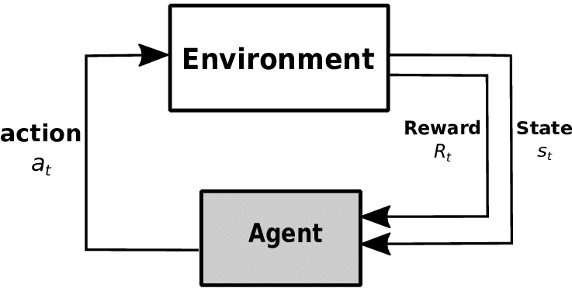
\includegraphics[width=8cm]{rl_example.png}
	\caption{Reinforcement learning problem formulation}
\end{figure}

\FloatBarrier

A policy is a probability distribution over actions given states. Given a policy $\pi$ the expected value of the current state $s \in S$ is the discounted sum of expected future rewards calculated by

\begin{align*}
	V^{\pi}\left(s_{t}\right)=\mathbb{E}_{\mathbb{P}}\left(\sum_{k \in \mathbb{N}} \gamma^{k} r_{t+k} \mid s_{t}, \pi\right)
\end{align*}

As the goal for the agent is to learn a policy that maximizes rewards the optimal value for a state is given by

\begin{align*}
	V^{\star}\left(s_{t}\right)=\max _{\pi \in \Pi}\left\{V^{\pi}\left(s_{t}\right)\right\}
\end{align*}

To compare action-state pairs in a policy the Q-value was proposed. This value is a measure of the expected future reward for taking a certain action in the current state in the current policy. The formulation is

\begin{align*}
	Q^{\pi}\left(s_{t}, a_{t}\right)=\mathbb{E}_{\mathbb{P}}\left[G_{t} \mid s_{t}, a_{t}, \pi\right]
\end{align*}

The optimal policy $\pi^*$ is one that select the highest Q-value action in every state, shown by

\begin{align*}
	\pi^{\star}\left(s_{t}\right)=\underset{a \in \mathcal{A}}{\operatorname{argmax}}\left\{Q^{\star}\left(s_{t}, a\right)\right\} .
\end{align*}

There are other important factors to consider when training a reinforcement learning agent. During training the agent needs to carefully balance exploration vs exploitation in order to ideally determine a globally optimal strategy. If there is no exploration the agent will stay in a local maxima, and if there is no exploitation the agent will act randomly. One common approach is to employ an $\epsilon$-greedy strategy where the agent will take a random action $\epsilon$ percent of the time. This parameter can we changed in order to highlight exploration or exploitation at any point during training.

\section{Assignment}

The objective of this assignment is to use reinforcement learning technique to design an algorithmic trading strategy on the Standard and Poor's 500 index EFT. The rules for the environment are as follows

\begin{itemize}
	\item[$-$] Initial portfolio value is \$10 on Jan. 3, 2012.
	\item[$-$] Short selling is allowed, but you cannot hold more than 2 units of the ETF short positions in your portfolio.
	\item[$-$] The transaction fee is 0.2\% for every trade.
	\item[$-$] You can only trade once per day.
	\item[$-$] You are not allowed to sell or buy more than 5 units per day either long or short.
\end{itemize}

The daily price data is provided in files train.csv and test.csv. The training data set is used in the training environment for the agent which is then evaluated using the testing data set in the testing environment to calculate the Sharpe ratio, cumulative returns, and return volatility. The target is to maximize the 3-month return while also minimizing the 3-month return volatility, which can be described as generating high and stable returns.

\section{Environment}

The environments are structured in a standard OpenAI gym format which takes actions as inputs and outputs information including the reward, the next state, and if the episode has terminated. Building on this framework there is an open-source library named FinRL that is specialized for the stock trading environment. The relevant RL problem formulation is as follows

\begin{itemize}
	\item Actions: The action space used is $(−k, ..., −1, 0, 1, ..., k)$, where k denotes the number of shares. For example, "Buy 10 shares of AAPL" or "Sell 10 shares of AAPL" are 10 or −10 respectively.
	\item Reward function: The change of the portfolio value when action $a$ is taken at state $s_t$ and arriving at new state $s_{t+1}$. The calculation is $R(s_t, a, s_{t+1}) = v_{t+1} − v$, where $v_{t+1}$ and $v$ represent the portfolio values at state $s_{t+1}$ and $s$ respectively.
	\item State: The state space for our agent is the current position, cash balance, and different trading signals that contain information for the agent to make decisions.
\end{itemize}

\section{Algorithms}

There are many algorithms to train DRL agents to solve a wide variety of tasks. Different types of algorithms have emerged, with the two major distinctions being online vs offline learning as well as model-based and model-free learning. In online learning the agent is interacting with the environment and collecting observations along the way, while offline learning takes observations from datasets and constructs a policy without the agent needing to run in the environment. In a model-based algorithm a forward model of the environment dynamics and the transition probabilities is constructed, while in a model-free algorithm there is no model of the environment constructed.

\subsection{DDQN}

Double Deep Q-Networks (DDQN) is an algorithm that adapts the concept of Deep Q-Learning (DQN) while addressing some known shortcomings. A Q-network is a network that takes any state-action pair $Q(s, a)$ and returns the expected future reward. DQN's utilize deep learning to calculate this expected reward and have been shown to be useful on a large variety of tasks. DDQN's were developed to address the problem of DQN overestimating Q values under certain conditions. This is addressed by having a separate network that executes the policy while another is used for training. Periodically the weights of the execution network is updated with the weights of the training network.

% \begin{figure}[h]
% 	\centering
% 	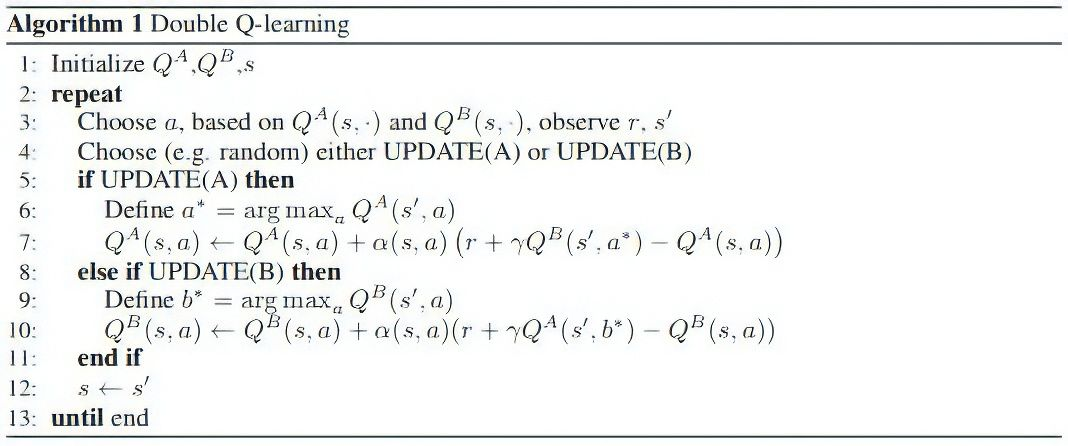
\includegraphics[width=14cm]{DQN_algo.png}
% 	% \caption{}
% \end{figure}

\FloatBarrier

\subsection{DDPG}

Deep Deterministic Policy Gradient (DDPG) is an algorithm which learns both a Q-function and a policy at the same time. It uses off-policy data to train a Q-network, and trains a policy network using the Q-network to maximize rewards. One main motivation of this approach is to address the problem with Q-learning methods that they only work for discrete actions and do no scale to large numbers of actions which can be very computationally expensive. Training this policy network addresses these problems and is a popular algorithm in many applications.

% \begin{figure}[h]
% 	\centering
% 	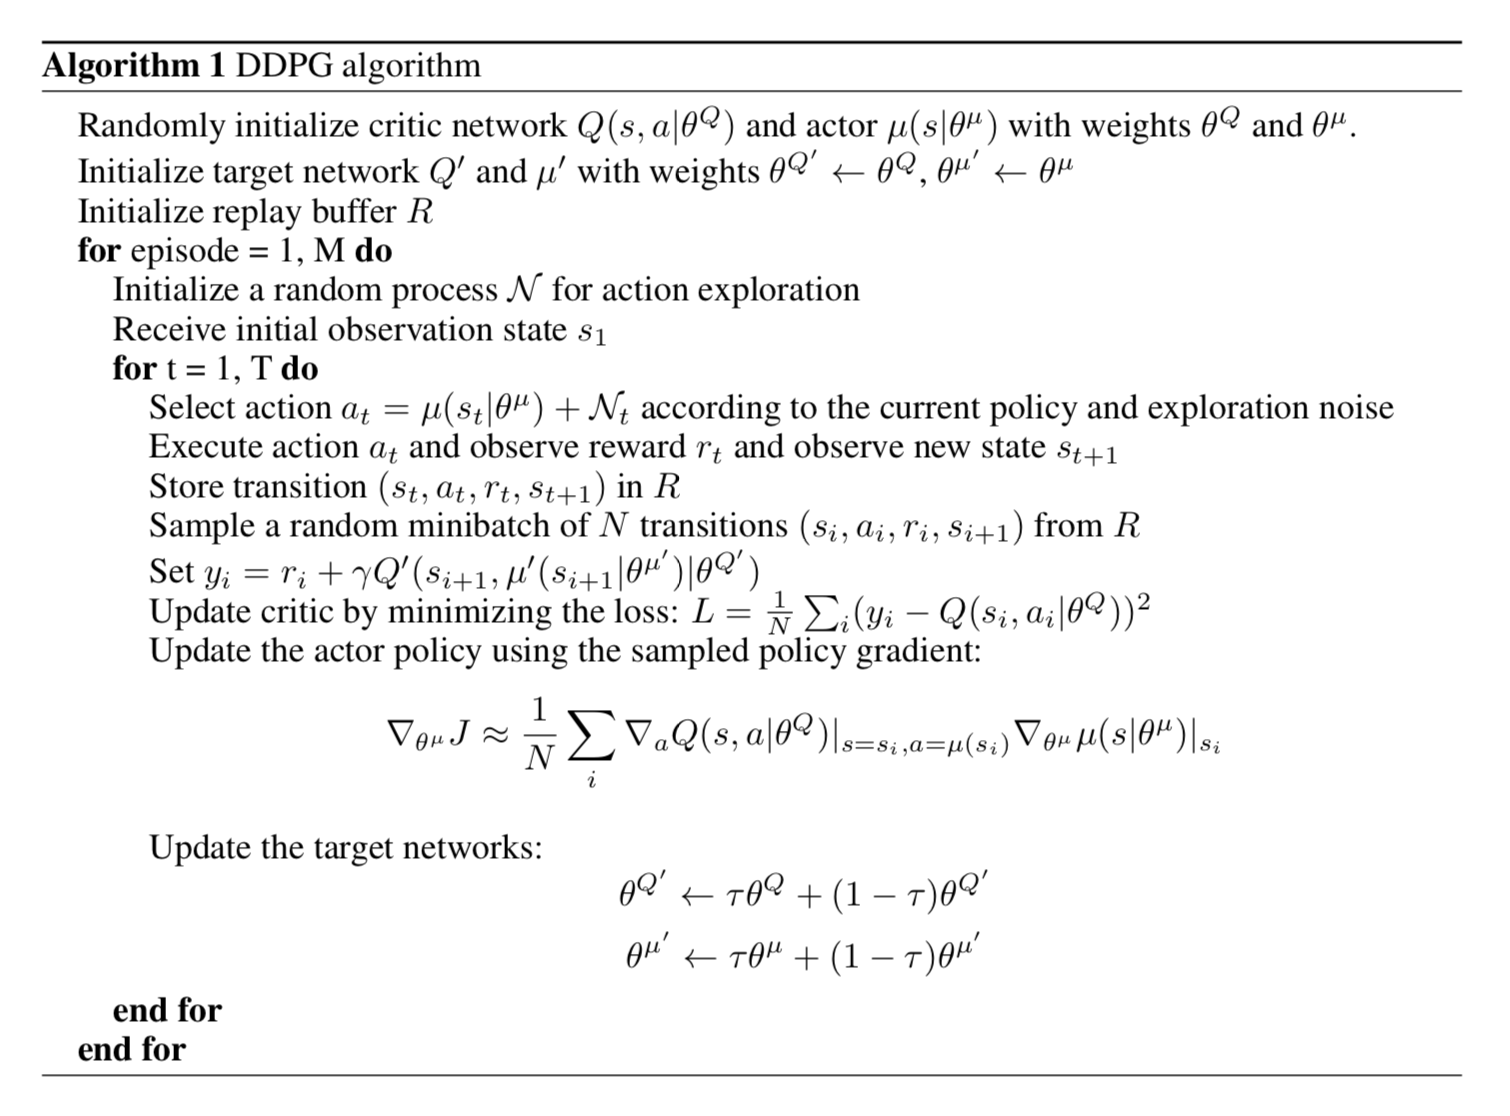
\includegraphics[width=14cm]{DDPG_algo.png}
% 	% \caption{Reinforcement learning problem formulation}
% \end{figure}

\section{Results}

The agents were run on the testing data and evaluated based on their average 3-month return and volatility. The following table consists of the results from both algorithms:

\begin{table}[h!]
	\centering
	\begin{tabular}{||c c c||}
		\hline
		Algorithm & 3-Month Returns & 3-Month Volatility \\ [0.5ex]
		\hline\hline
		DDQN      & 0.49\%          & 1.45\%             \\
		DDPG      & 2.87\%          & 1.46\%             \\ [1ex]
		\hline
	\end{tabular}
	\caption{Simulation results per algorithm}
	\label{table:1}
\end{table}

\section{Future Work}

This project was an initial look at using reinforcement learning in a single stock trading environment. There are a number of ways to improve this analysis in future work

\begin{itemize}
	\item Increase the granularity of the data from daily to hour, minute, or tick level data.
	\item Test other model configurations that would also be enabled with more granular data such as recurrent neural networks (RNNs).
	\item Use more recent DRL algorithms such as Twin Delay DDPG (TD3) which is an improvement over the DDPG algorithm used in this paper.
	\item Another possibility is to frame the problem as a continuous portfolio optimization problem rather than discretely buying individual stocks.
\end{itemize}

\section{Code}

All the code is available online at \url{https://github.com/mvkvc/RL_trading}. The data is hosted at and experiments were run at \url{https://dagshub.com/mvkvc/RL_trading}. These results can be recreated by following the instruction in the README.

\end{document}